\documentclass[12pt,a4paper]{scrartcl}
\usepackage[utf8]{inputenc}
\usepackage[english,russian]{babel}
\usepackage{indentfirst}
\usepackage{misccorr}
\usepackage{graphicx}
\usepackage{amsmath}
\usepackage{multirow}
\usepackage{pgfplots}
\usepackage{parskip}
\usepackage[top=1cm, bottom=1cm, left=1cm, right=1cm]{geometry}
\pgfplotsset{compat=1.9}

\begin{document}
	\graphicspath{{pic/}, {~/Pictures/TeXImgs/}}
	
	\newcommand{\ms}{\mathstrut}
	\newcommand{\msp}{\hspace{0.5cm}}
	\newcommand{\al}{\alpha}
	\newcommand{\dg}{^\circ}
	\newcommand{\dif}{\mathrm{d}}
	\newcommand{\qd}[2]{^{\frac{#1}{#2}}}
	\newcommand{\qdm}[2]{^{-\frac{#1}{#2}}}
	\newcommand{\lm}[2]{\underset{#1 \rightarrow #2}{\lim}}
	\newcommand{\sfrac}[2]{\dfrac{\strut #1}{\strut #2}}
	\newcommand{\equal}[1]{\overset{(#1)}{=}}
	\newcommand{\linevdots}{\ \raisebox{-.08\height}{\vdots}\ }
	\newcommand{\linecvdots}{\ \raisebox{-.08\height}{\vdots}\hspace{-0.13cm}\raisebox{.15\height}{\cancel{\phantom{a}}\hspace{0.06cm}}}
	\newcommand{\combox}[1]{\ms \msp \msp \begin{minipage}{0.95\linewidth}
			#1
	\end{minipage}}
	
	\newtheorem{pr}{Задача}
	\newtheorem{ex}{Пример}
	\newtheorem{dfn}{Def}
	\newtheorem{theorem}{Th}
	
	\newenvironment{slv}{\ms \msp \textit{Решение:}}{}
	\newenvironment{proof}{\ms \msp \textit{Доказательство: }}{\hfill $\square$}
	
	\begin{titlepage}
		
		\vspace*{\fill}
		
		\begin{center}
			
\includegraphics[scale=0.8]{MIPT.png}
			\\[0.7cm]\Huge Московский Физико-Технический Институт\\(национальный исследовательский университет)
			\\[2cm]\LARGE Отчет по эксперименту
			\\[0.5cm]\noindent\rule{\textwidth}{1pt}
			\\\Huge\textbf{Измерение коэффициента поверхностного натяжения жидкости}
			\\[-0.5cm]\noindent\rule{\textwidth}{1pt}
		\end{center}
		
		\begin{flushleft}
			\textit{Работа №2.5.1; дата: 08.04.22}\hfill\textit{Семестр: 2}
		\end{flushleft}
		
		\vspace*{\fill}
		
		\begin{flushleft}
			Выполнил: \hspace{\fill} Группа:
			\\Кошелев Александр \hspace{\fill} Б05-105
		\end{flushleft}
	\end{titlepage}
	
	%Страница 2
	
	\begin{flushleft}
		\footnotesize{Измерение коэффициента поверхностного натяжения жидкости} \hspace{\fill} \footnotesize{2}
		\\[-0.3cm]\noindent\rule{\textwidth}{0.3pt}
	\end{flushleft}
	
	\section{Аннотация}
	
	\textbf{Цель работы: }
	
	\begin{enumerate}
		\item Измерение температурной зависимости коэффициента поверхностного натяжения дистиллированной воды с использованием известного коэффициента поверхностного натяжения спирта
		\item Определение полной поверхностной энергии  и теплоты, необходимой для изотермического образования единицы  поверхности жидкости  при различной температуре
	\end{enumerate}
	
	\textbf{Схема установки:}
	\begin{center}
		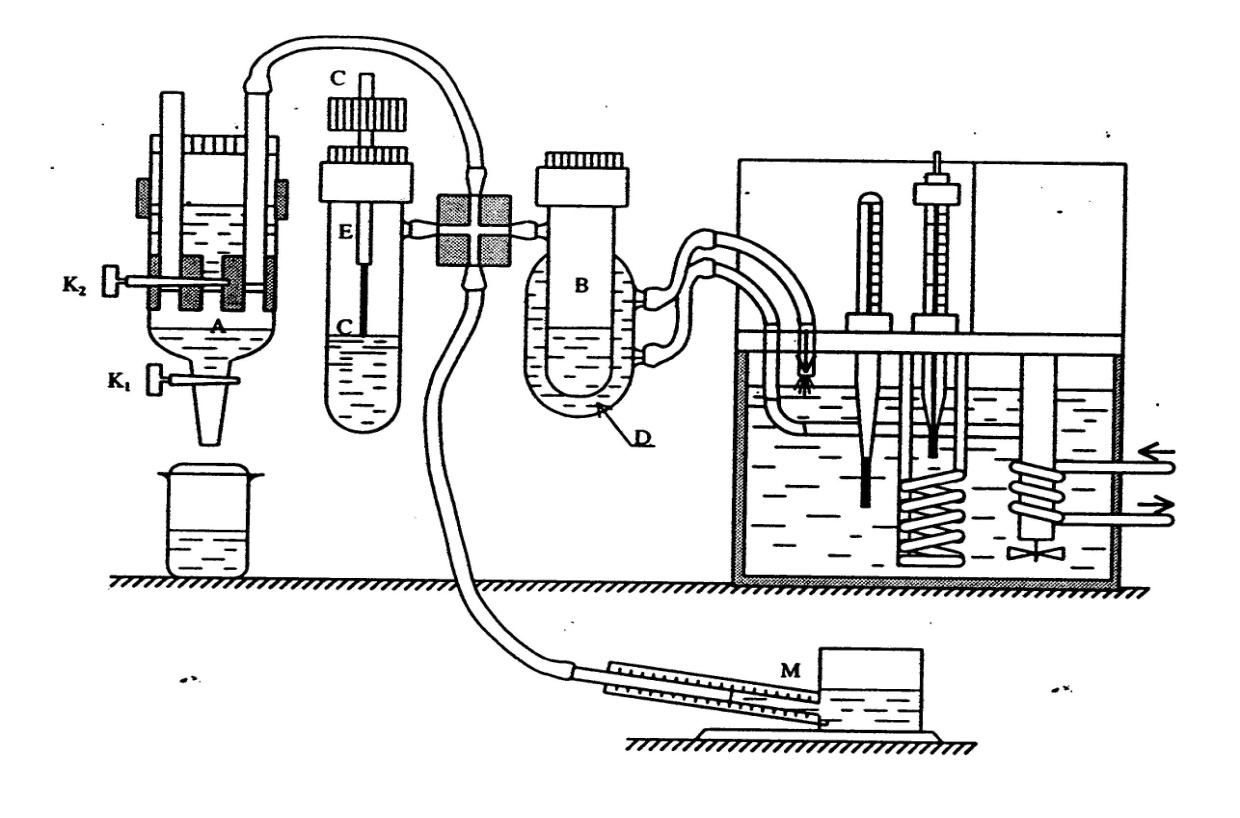
\includegraphics[scale=0.3]{PIC_1.png}
		\\\textbf{Рис. 1:} Схема установки
	\end{center}
		
	Исследуемая жидкость (дистиллированная вода) наливается в сосуд (колбу) $B$. Тестовая жидкость (этиловый спирт) наливается в сосуд $E$. При измерениях колбы герметично закрываются пробками. Через одну из двух пробок проходит полая металлическая игла $C$. Этой пробкой закрывается сосуд, в котором проводятся измерения. Верхний конец иглы открыт в атмосферу, а нижний погружен в жидкость. Другой сосуд герметично закрывается второй пробкой. При создании достаточного разрежения воздуха в колбе с иглой пузырьки воздуха начинают пробулькивать через жидкость. Поверхностное натяжение можно определить по величине разряжения $\Delta P$, необходимого для прохождения пузырьков (при известном радиусе иглы). Разрежение в системе создается с помощью аспиратора $A$. Кран $K_2$ разделяет две полости аспиратора. Верхняя полость при закрытом кране $K_2$ заполняется водой. Затем кран $K_2$ открывают и заполняют водой нижнюю полость  аспиратора. Разрежение воздуха создается в нижней полости при открывании крана $K_1$, когда вода вытекает из неё по каплям. В колбах $B$ и $C$, соединённых трубками с нижней полостью аспиратора, создается такое же пониженное давление. Разность давлений в полостях с разреженным воздухом и атмосферой измеряется спиртовым микроманометром. Для стабилизации температуры исследуемой жидкости через рубашку $D$ колбы $B$ непрерывно прогоняется вода из термостата.	
		
	\textbf{В работе используются:}
	
	Прибор Ребиндера с термостатом и микроманометром, исследуемые жидкости, стаканы.
	
	\section{Теоретические сведения}
	Наличие поверхностного слоя приводит к различию давлений по разные стороны от искривленной границы раздела двух сред. Для сферического пузырька с воздухом внутри жидкости избыточное давление даётся формулой Лапласа:
	
	\newpage 
	
	%Страница 3
	
	\begin{flushleft}
		\footnotesize{Измерение коэффициента поверхностного натяжения жидкости} \hspace{\fill} \footnotesize{3}
		\\[-0.3cm]\noindent\rule{\textwidth}{0.3pt}
	\end{flushleft}
	
	$$\Delta P = P_{\text{внутри}} - P_{\text{снаружи}} = \sfrac{2 \sigma}{R}$$
	
	Где $\sigma$ -- коэффициент поверхностного натяжения, $_{\text{внутри}}$ и $P_{\text{снаружи}}$ -- давление внутри пузырька и снаружи, $R$ -- радиус кривизны поверхности раздела двух фаз. Эта формула лежит в основе предлагаемого метода определения коэффициента поверхностного натяжения жидкости. Измеряется давление $\Delta P$, необходимое для выталкивания в жидкость пузырька воздуха.

	\section{Проведение эксперимента}
	\paragraph{Основные параметры при проведении эксперимента} \hfill
	
	Основными параметрами в данной ряботе являются плотность эталонной жидкости -- этанола $\rho_0 = 809.5$ кг/м$^3$, плотность исследуемой жидкости -- воды $\rho = 998.2$ кг/м$^3$, ускорение свободного падения $g = 9.81$ м/с$^2$, пересчетный коэффициент $k = 0.2$, коэффициент поверхностного натяжения этанола $\sigma_0 = 22.75$ мН/м.
	
	\paragraph{Измерение диаметра иглы} \hfill
	
	Вначале двумя способами оценим диаметр иглы. Первый -- прямое измерение микроскопом, при этом получаем $d = (1.05 \pm 0.05)$ мм. Второй -- по известному коэффициенту поверхностного натяжения спирта.

	\begin{center}
		\begin{tabular}{|c|c|c|c|c|c|c|}
			\hline
			$i$ & 1 & 2 & 3 & 4 & 5 & среднее
			\\\hline
			$P$, дел & $47.0 \pm 0.5$ & $47.0 \pm 0.5$ & $47.0 \pm 0.5$ & $47.0 \pm 0.5$ & $47.0 \pm 0.5$ & $47.0 \pm 0.5$
			\\\hline
			$\overline{P}$, Па & \multicolumn{6}{|c|}{$92.18 \pm 0.98$}
			\\\hline
			$d$, мм & \multicolumn{6}{|c|}{$0.99 \pm 0.01$}
			\\\hline
		\end{tabular}
		\\\textbf{Табл. 1:} Измерение диаметра иглы
	\end{center}

	Как видно из полученных значений, они совпадают в пределах стандартного отклонения.

	\paragraph{Проверка соотношения давлений} \hfill

	Вначале установим иглу у поверхности воды, а затем опустим ее в глубь воды. При этом соответствующие высоту иглы от неподвижной части установки $h_1 = 1.85 \pm 0.05$ см, $h_2 = 0.65 \pm 0.05$ см. Получаем первое из значений $\Delta h = 1.2 \pm 0.1$ см. Измерения давлений занесем в таблицу:
	
	\begin{center}
		\begin{tabular}{|c|c|c|c|c|c|c|}
			\hline
			$i$ & 1 & 2 & 3 & 4 & 5 & среднее
			\\\hline
			$P_1$, дел & $140.0 \pm 0.5$ & $140.0 \pm 0.5$ & $140.0 \pm 0.5$ & $140.0 \pm 0.5$ & $140.0 \pm 0.5$ & $140.0 \pm 0.5$
			\\\hline
			$P_2$, дел & $204.0 \pm 0.5$ & $204.0 \pm 0.5$ & $204.0 \pm 0.5$ & $204.0 \pm 0.5$ & $204.0 \pm 0.5$ & $204.0 \pm 0.5$
			\\\hline
			$\Delta P$, дел & $64 \pm 1$ & $64 \pm 1$ & $64 \pm 1$ & $64 \pm 1$ & $64 \pm 1$ & $64 \pm 1$
			\\\hline
			$\Delta h$, мм & \multicolumn{6}{|c|}{$1.3 \pm 0.1$}
			\\\hline
		\end{tabular}
		\\\textbf{Табл. 2:} Проверка соотношения давлений
	\end{center}

	Вновь наблюдаем совпадение сопоставляемых значений с точностью в пределах стандартного отклонения. Здесь же из формулы 1 рассчитаем коэффициент поверхностного натяжения воды при 20 $^\circ$C:
	$$\sigma = \sfrac{P}{P_0} \sigma_0 = (67.8 \pm 0.76)\, \text{мН}/\text{м}$$
	
	\newpage
	
	%Страница 4
	
	\begin{flushleft}
		\footnotesize{Измерение коэффициента поверхностного натяжения жидкости} \hspace{\fill} \footnotesize{4}
		\\[-0.3cm]\noindent\rule{\textwidth}{0.3pt}
	\end{flushleft}
	
	\paragraph{Определение температурного коэффициента} \hfill
	
	Оформим полученные данные в виде таблицы.
	
	\begin{center}
		\begin{tabular}{|c|c|c|c|c|c|c|}
			\hline
			$t, ^\circ$C & \multicolumn{5}{|c|}{$P$, дел} & $\overline{P}$, дел
			\\\hline
			$20.0 \pm 0.1$ & $204.0 \pm 0.5$ & $203.0 \pm 0.5$ & $204.0 \pm 0.5$ & $204.0 \pm 0.5$ & $204.0 \pm 0.5$ & $203.8 \pm 0.5$
			\\\hline
			$24.2 \pm 0.1$ & $203.0 \pm 0.5$ & $203.0 \pm 0.5$ & $203.0 \pm 0.5$ & $204.0 \pm 0.5$ & $203.0 \pm 0.5$ & $203.2 \pm 0.5$
			\\\hline
			$29.6 \pm 0.1$ & $202.0 \pm 0.5$ & $202.0 \pm 0.5$ & $202.0 \pm 0.5$ & $202.0 \pm 0.5$ & $202.0 \pm 0.5$ & $202.0 \pm 0.5$
			\\\hline
			$35.5 \pm 0.1$ & $201.0 \pm 0.5$ & $201.0 \pm 0.5$ & $201.0 \pm 0.5$ & $201.0 \pm 0.5$ & $201.0 \pm 0.5$ & $201.0 \pm 0.5$
			\\\hline
			$41.4 \pm 0.1$ & $199.0 \pm 0.5$ & $199.0 \pm 0.5$ & $199.0 \pm 0.5$ & $199.0 \pm 0.5$ & $199.0 \pm 0.5$ & $199.0 \pm 0.5$
			\\\hline
			$44.3 \pm 0.1$ & $198.0 \pm 0.5$ & $198.0 \pm 0.5$ & $198.0 \pm 0.5$ & $197.0 \pm 0.5$ & $198.0 \pm 0.5$ & $197.8 \pm 0.5$
			\\\hline
			$50.3 \pm 0.1$ & $195.0 \pm 0.5$ & $195.0 \pm 0.5$& $195.0 \pm 0.5$ & $195.0 \pm 0.5$ & $195.0 \pm 0.5$ & $195.0 \pm 0.5$
			\\\hline
			$56.0 \pm 0.1$ & $193.0 \pm 0.5$ & $194.0 \pm 0.5$ & $194.0 \pm 0.5$ & $193.0 \pm 0.5$ & $193.0 \pm 0.5$ & $193.6 \pm 0.5$
			\\\hline
			$59.0 \pm 0.1$ & $193.0 \pm 0.5$ & $193.0 \pm 0.5$ & $193.0 \pm 0.5$ & $193.0 \pm 0.5$ & $193.0 \pm 0.5$ & $193.0 \pm 0.5$
			\\\hline
		\end{tabular}
		\\\textbf{Табл. 3:} Зависимость $P(t)$
	\end{center}
	
	На основе этих данных построим график, и определим тепературный коэффициент для коэффициента поверхностного натяжения.
	
	\begin{center}
		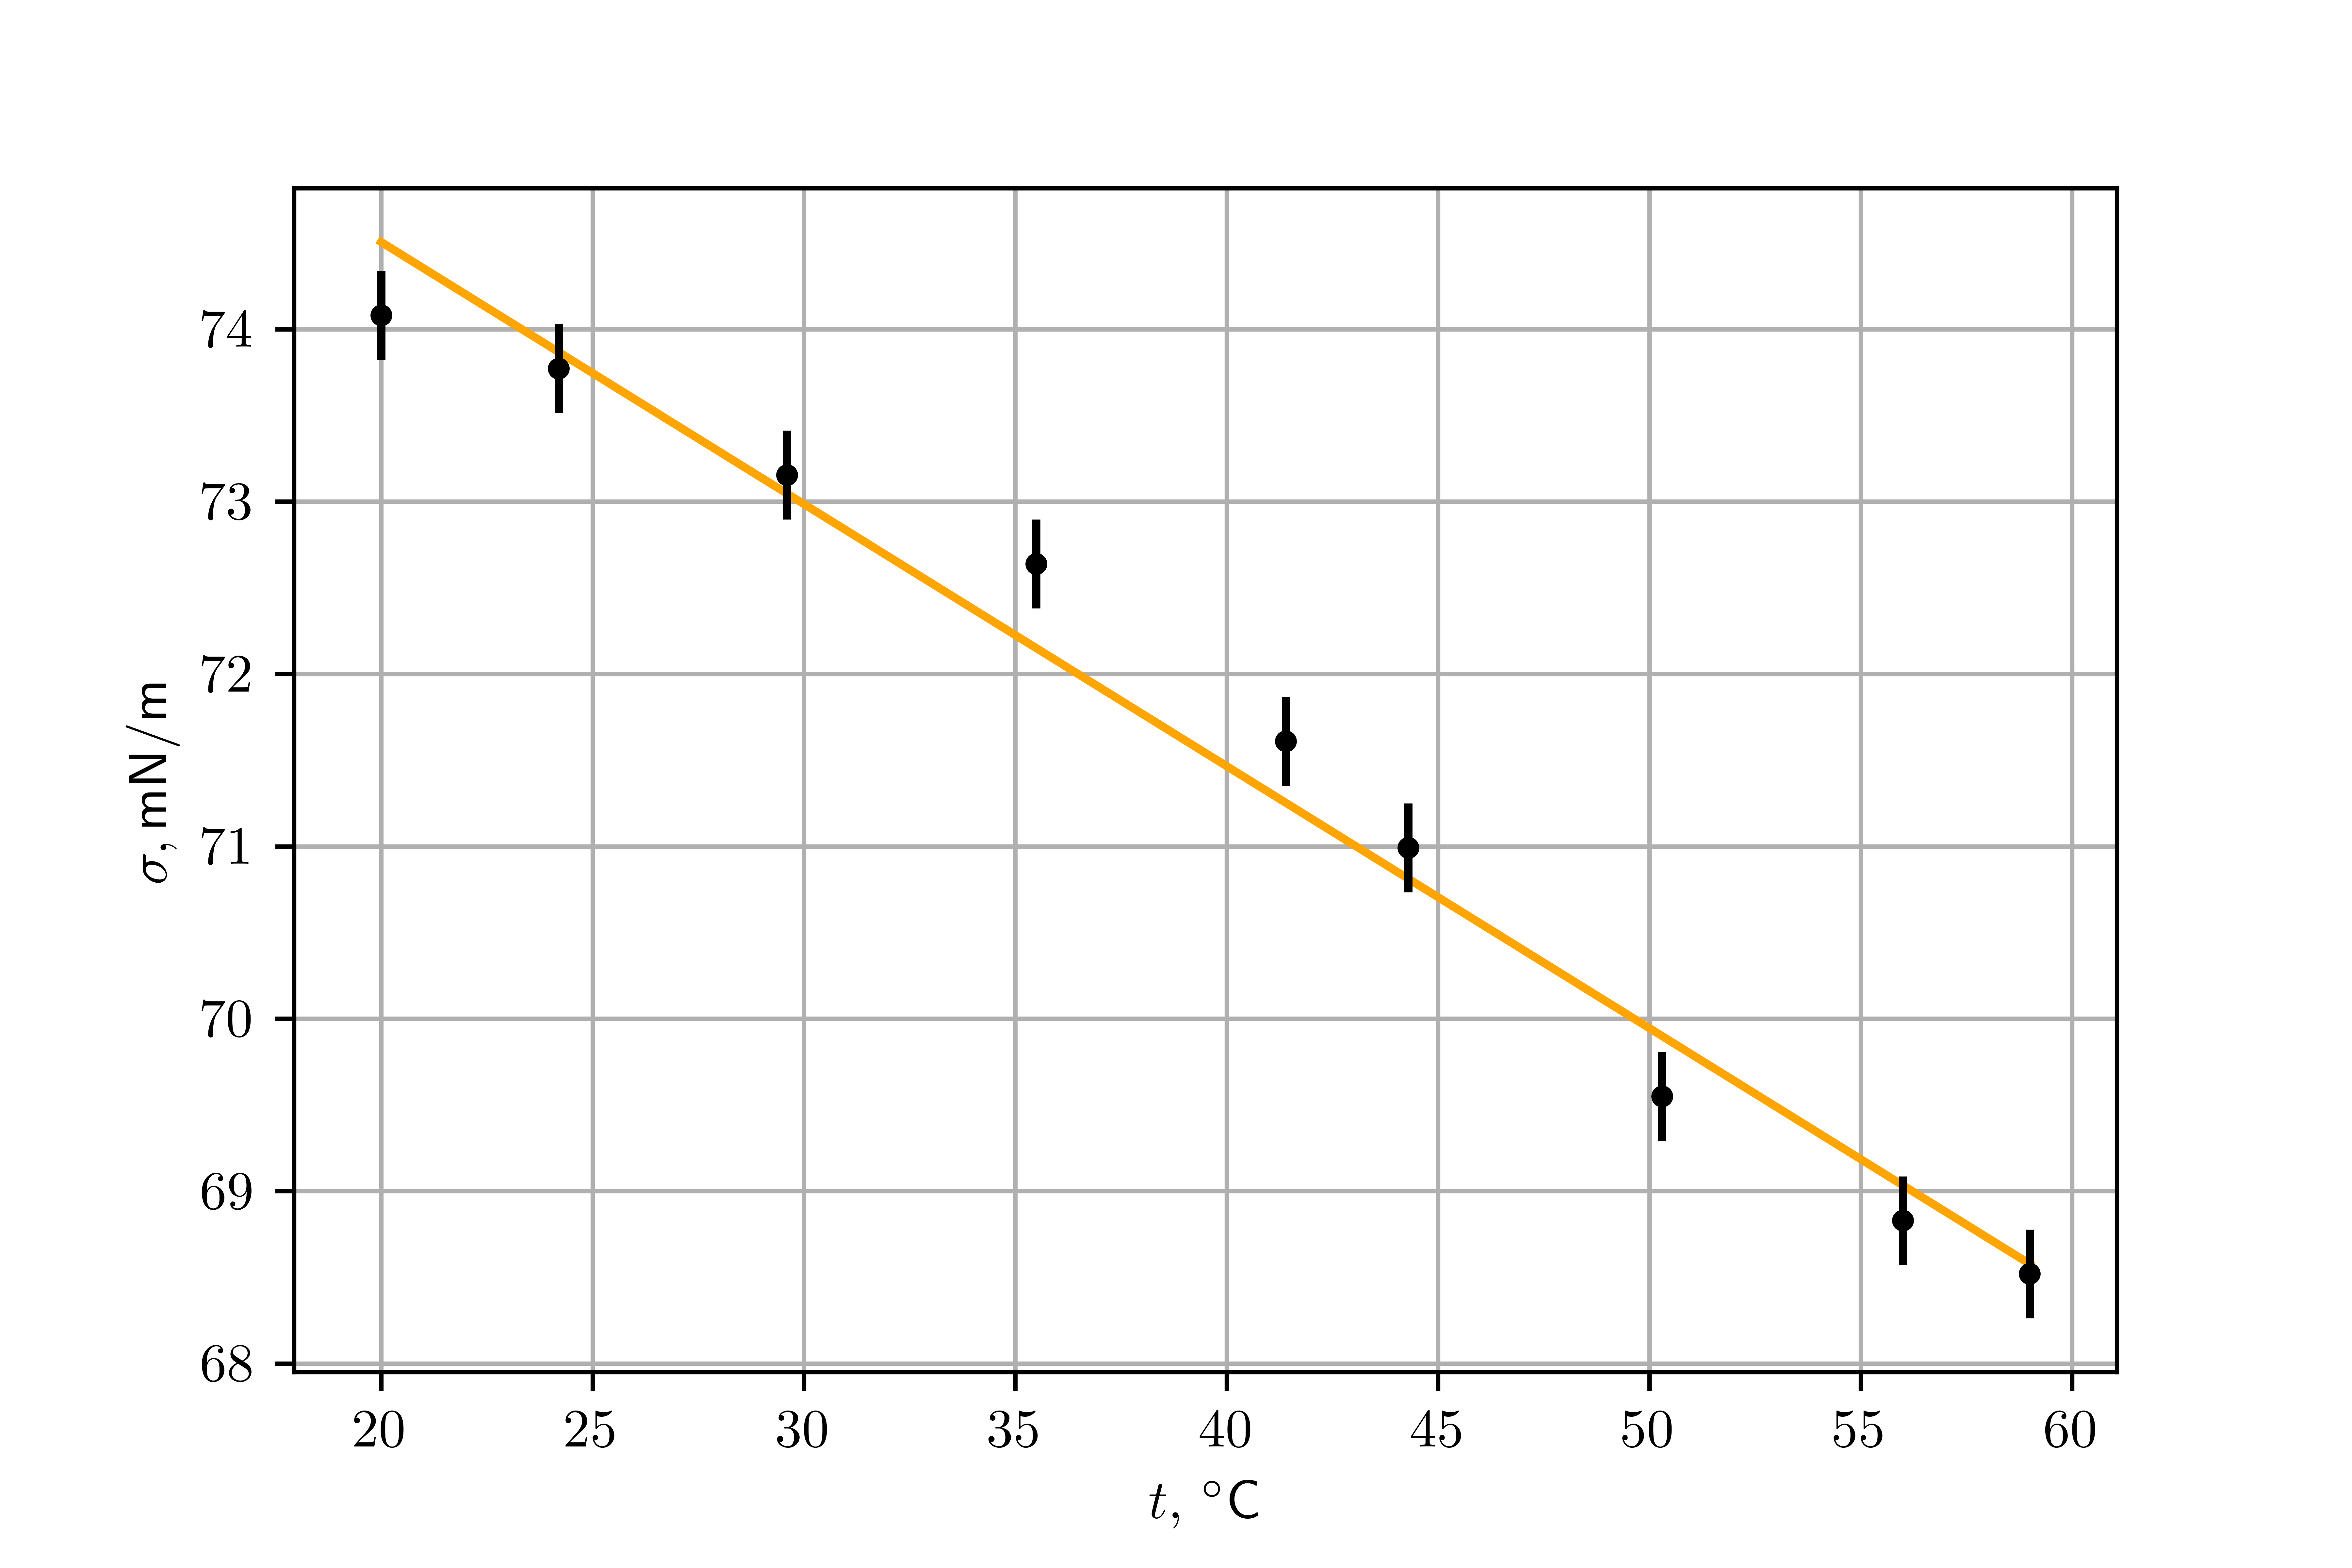
\includegraphics[scale=1]{PIC_2.png}
		\\\textbf{Рис. 2:} График зависимости $\sigma(t)$
	\end{center}

	$$\sfrac{\dif \sigma}{\dif T} = (-0.152 \pm 0.008)\, \sfrac{\text{мН}}{\text{м} \cdot \text{К}}$$
	
	\newpage
	
	%Страница 5
	
	\begin{flushleft}
		\footnotesize{Измерение коэффициента поверхностного натяжения жидкости} \hspace{\fill} \footnotesize{5}
		\\[-0.3cm]\noindent\rule{\textwidth}{0.3pt}
	\end{flushleft}
	
	\paragraph{Построение оставшихся графиков}	\hfill
	
	В этом пункте приведем графики зависимости теплоты образования единицы поверхности и энергии образования единицы поверхности.
	
	\begin{center}
		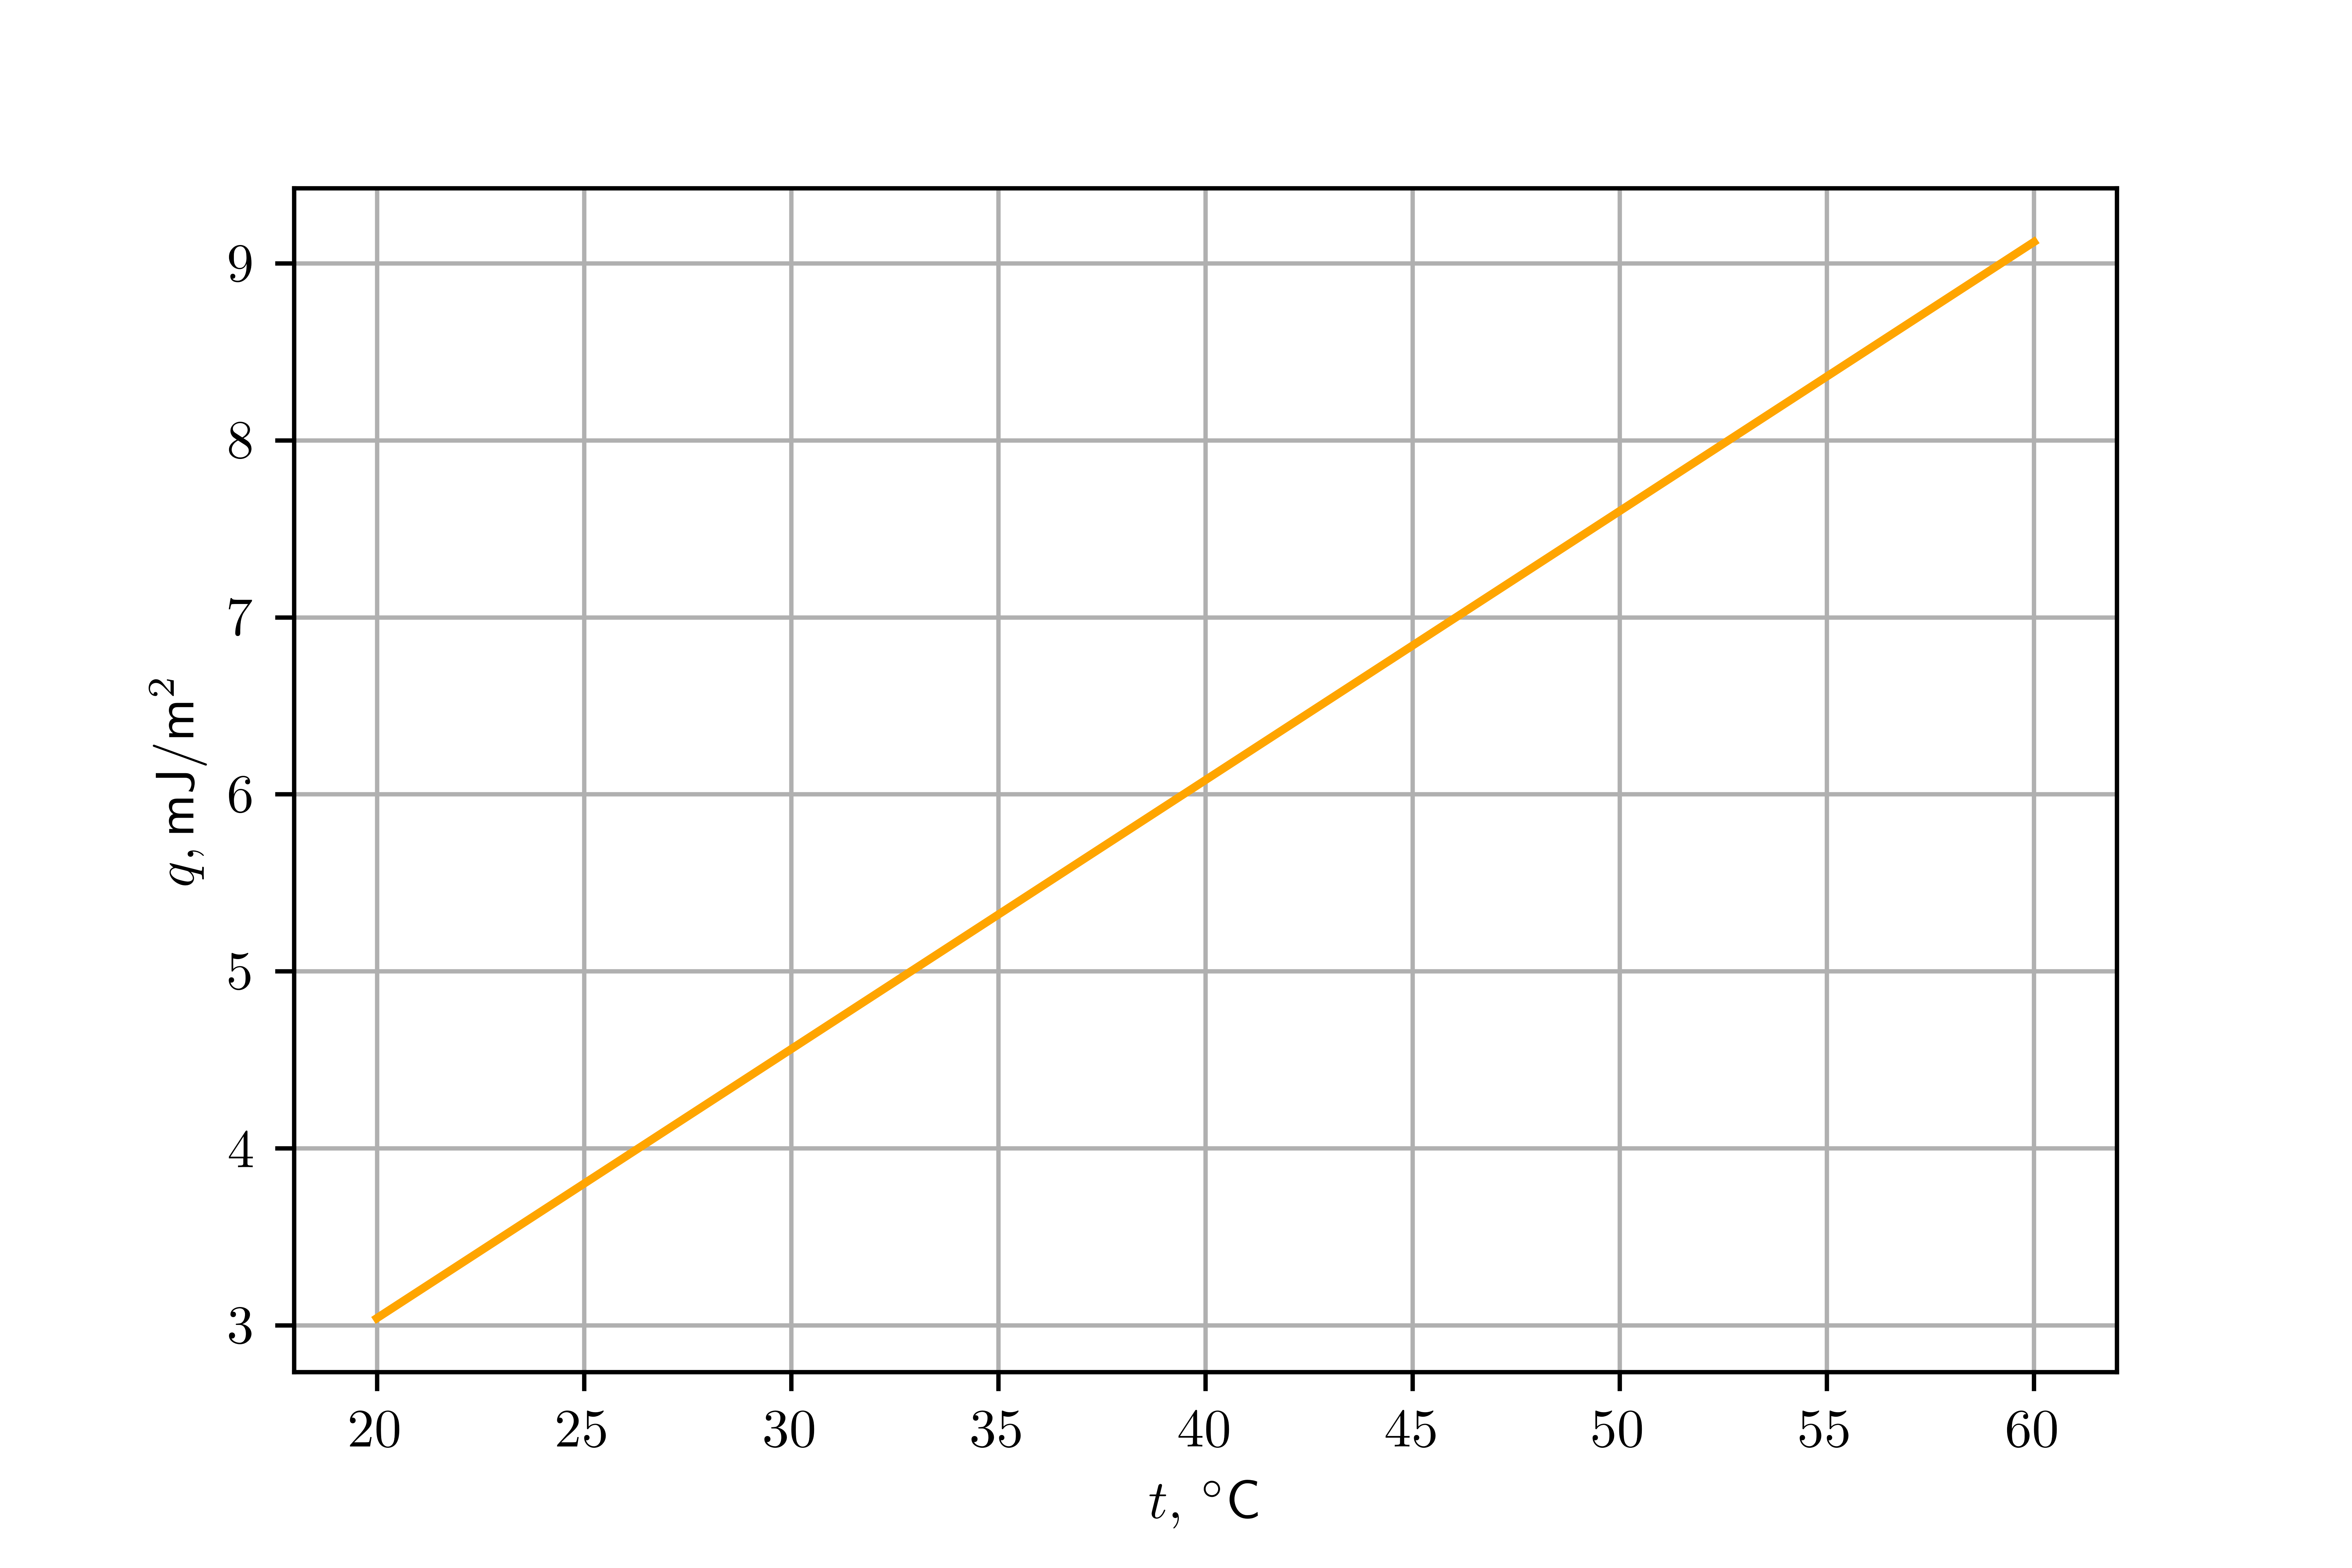
\includegraphics[scale=1]{PIC_3.png}
		\\\textbf{Рис. 3:} График зависимости $q(t)$
	\end{center}
	
	\begin{center}
		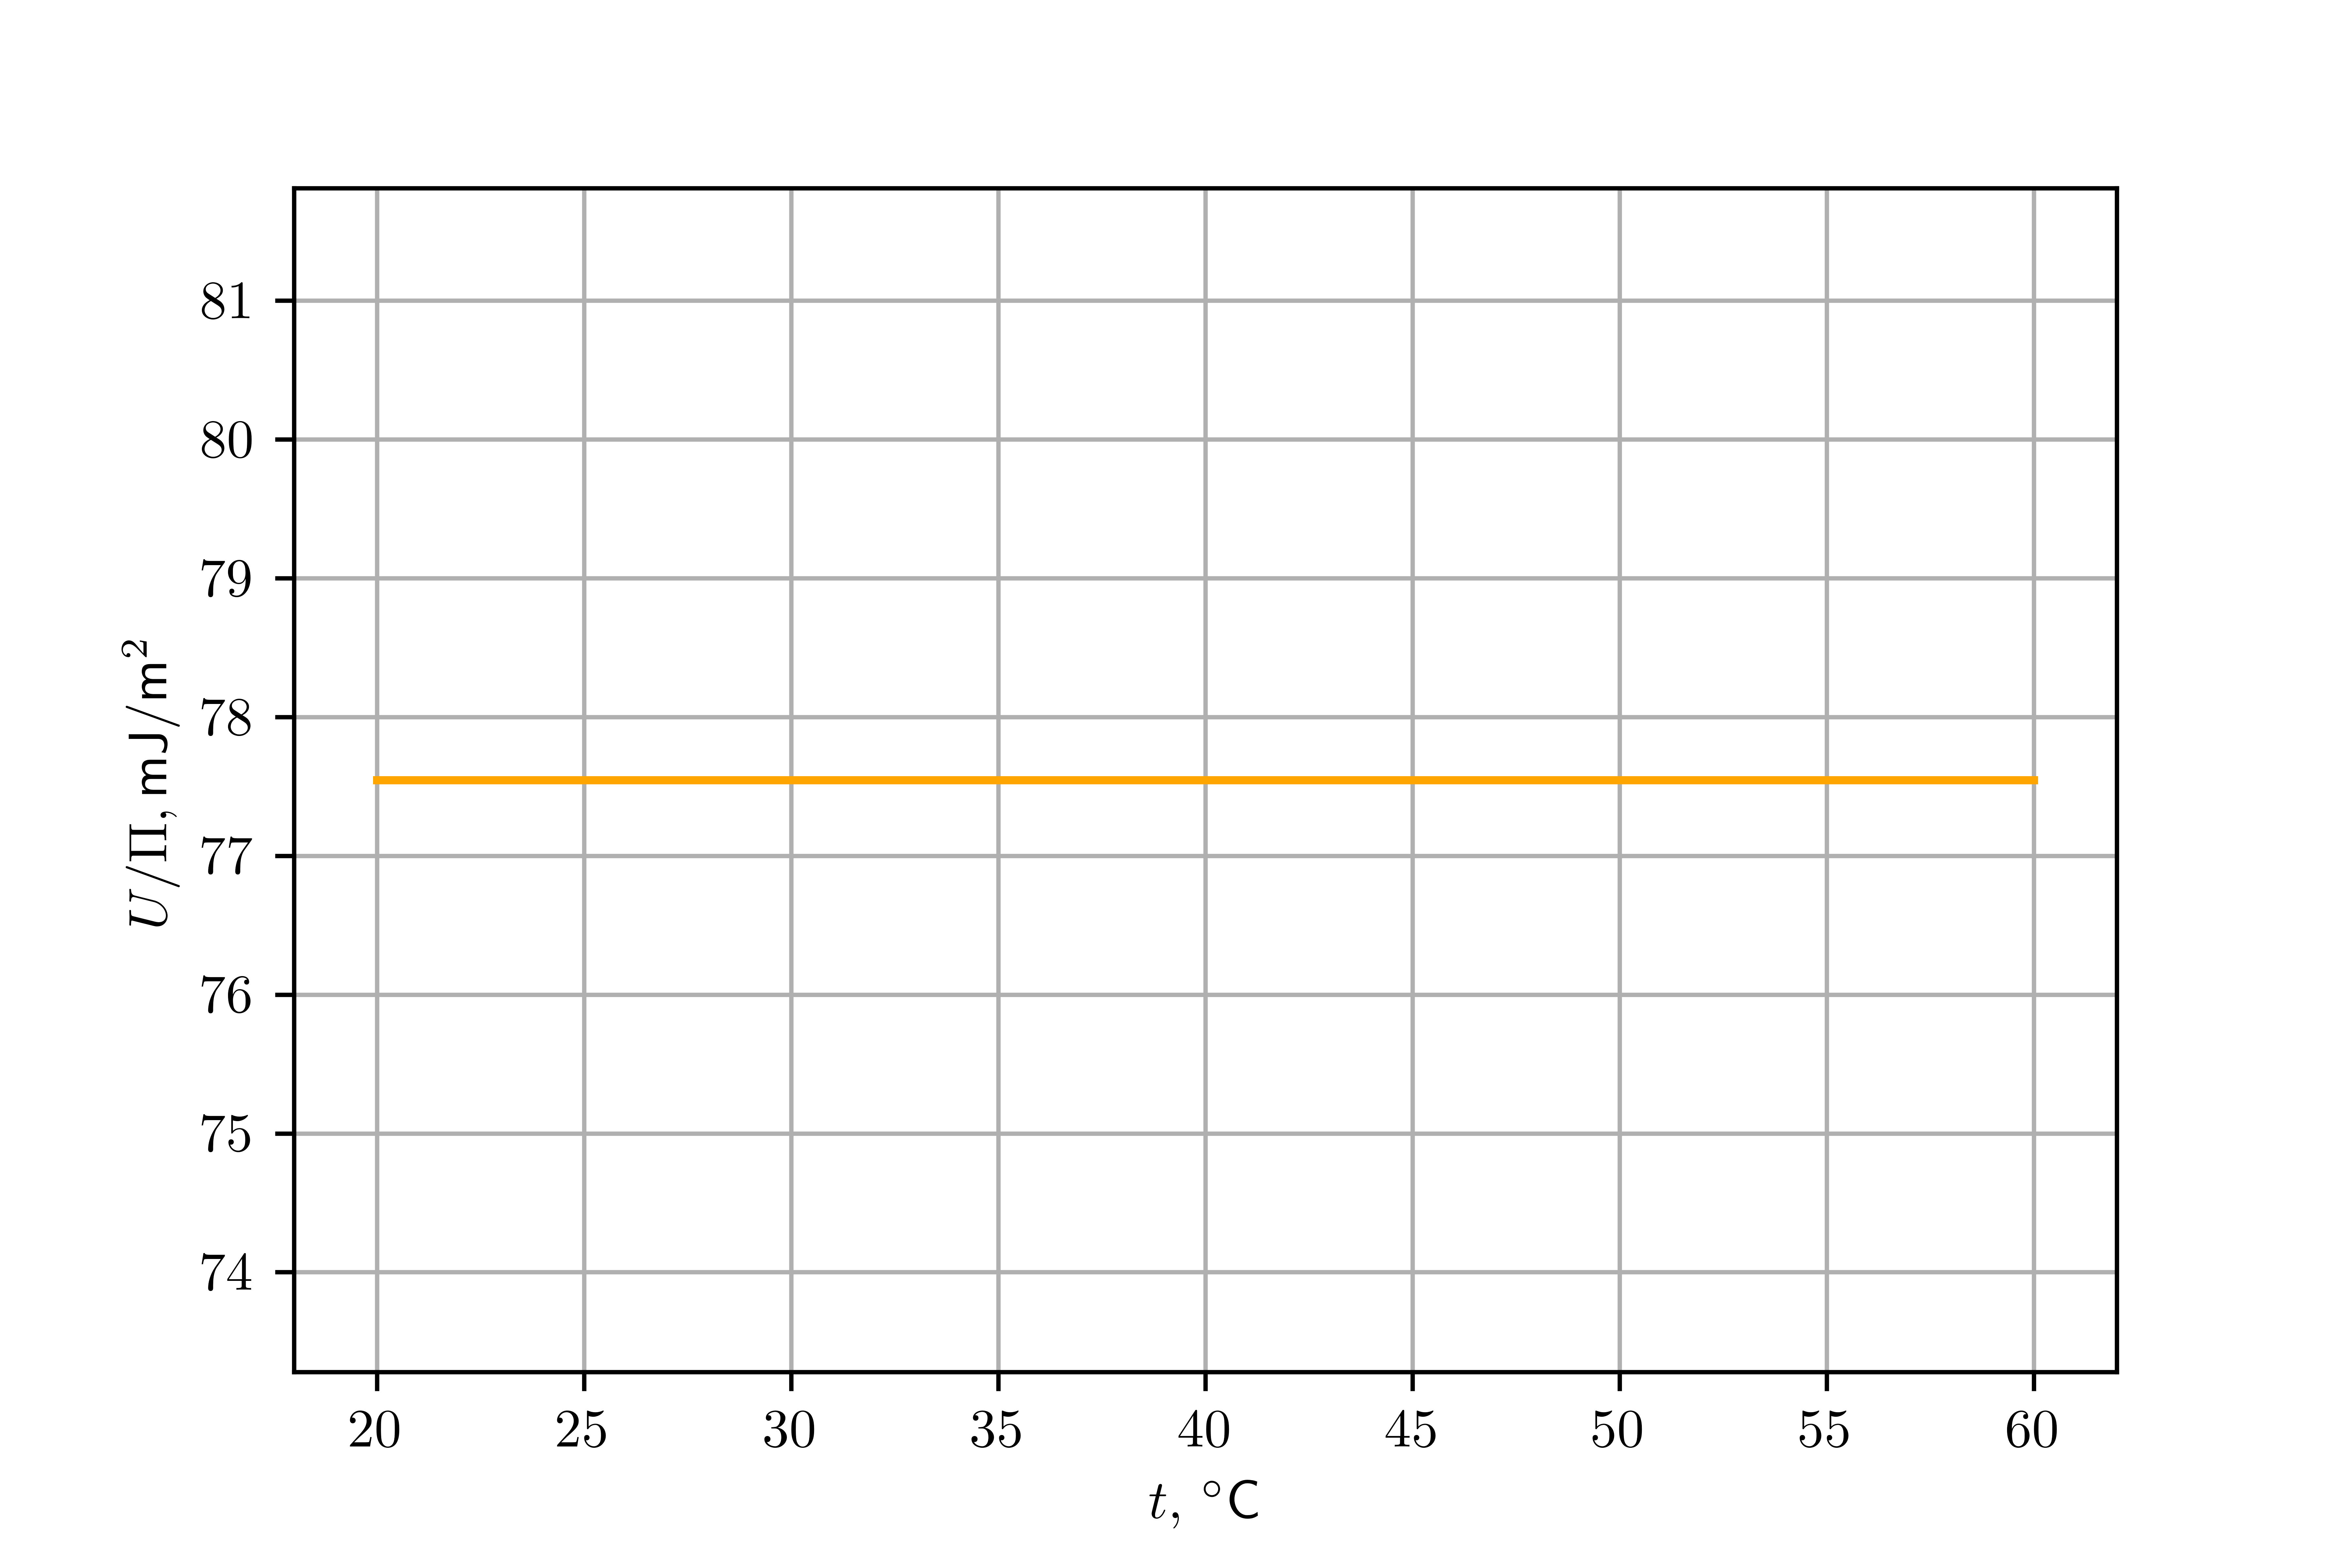
\includegraphics[scale=1]{PIC_4.png}
		\\\textbf{Рис. 4:} График зависимости $U/\Pi(t)$
	\end{center}
	
	\newpage
	
	%Страница 6
	
	\begin{flushleft}
		\footnotesize{Измерение коэффициента поверхностного натяжения жидкости} \hspace{\fill} \footnotesize{6}
		\\[-0.3cm]\noindent\rule{\textwidth}{0.3pt}
	\end{flushleft}
	
	\section{Выводы}
	\begin{enumerate}
		\item В результате работы определено, что в нашем диапазоне температур зависимость коэффициента поверхностного натяжения воды от температуры линейна, приичм убывает. Соответствующий коэффициент:
		
		$$\left|\sfrac{\dif \sigma}{\dif T}\right| = (0.152 \pm 0.008)\, \sfrac{\text{мН}}{\text{м} \cdot \text{К}}$$
		
		Что близко к табличному значению $\alpha = 0.154\, \frac{\text{мН}}{\text{м} \cdot \text{К}}$ в пределах стандартного отклонения.
		
		\item Получены зависимости теплоты и энергии образования единицы поверхности жидкости при данных температурах. Они приведены на Рис. 3-4.
	\end{enumerate}
	
\end{document}